%\documentclass[a4paper, 12pt, twoside]{Thesis}% 
\documentclass[a4paper, 12pt, oneside]{Thesis}%ITS ONESIDE NOW JUST FOR EDITING

\usepackage[draft]{todonotes}   % notes showed

%THIS PACKAGES ARE FROM TEMPLATE DONT TOUCH!!!!!!!!!!!!!!!!!!
\usepackage{graphicx}
\usepackage{verbatim}
\usepackage[english]{babel}
\usepackage[utf8]{inputenc}
\usepackage[T1]{fontenc}
\usepackage{algorithmic}
\usepackage{algorithm}
\usepackage{pdfpages}
\usepackage{time}
\usepackage{appendix}
\usepackage{sidecap}
\setlength{\parindent}{0.25in}
\hypersetup{urlcolor=blue, colorlinks=false}
%THIS PACKAGES ARE FROM TEMPLATE DONT TOUCH!!!!!!!!!!!!!!!!!!


\def \listfigures {List of Figures}

\def \university {University Institute of Lisbon}
\def \department {Department of Information Science and Technology}

\def \supervisortitle {Supervisor}
\def \supervisorname  {Prof. João Carlos Amaro Ferreira, PhD}
\def \supervisoruniv{ISCTE-IUL}

\def \cosupervisortitle {Co-Supervisor}
\def \cosupervisorname {Rui Maia, PhD}
\def \cosupervisoruniv {Instituto Superior Técnico}

\def \dissertationstatement {Relatório do Estado da Arte para:}
\def \dissertationtitle {Introdução à Investigação em Engenharia }

\begin{document}

\frontmatter

\title  {Vessel Behavior Analysis}
\authors  {Tomás Manuel Cardoso Machado}
            
\addresses  {\groupname\\\deptname\\\univname}
\date       {January 2018}
\subject    {}
\keywords   {}
\maketitle

\fancyhead{}
%\fancyfoot[LE,RO]{\thepage} %PAGE NUMBER TO PRINT AFTER...
\fancyfoot[C]{\thepage}
\lhead{}

\pagestyle{fancy}


%-------ABSTRACT---------
%\cleardoublepage
%\addtotoc{Abstract}
%\abstract{

%Abstract text

%\textbf{Keywords:} Keyword1, Keyword2.
%}

%\cleardoublepage
%\setstretch{1.3}

%-------IDIOMA DA TESE---------
\selectlanguage{english}

%-------ÍNDICE---------
\lhead{\emph{Contents}}
\tableofcontents

%-------LISTA DE FIGURAS---------
%\lhead{\emph{List of Figures}} 
%\listoffigures 

%-------LISTA DE TABELAS---------
%\lhead{\emph{List of Tables}} 
%\listoftables 

%-------LISTA DE TODOS---------
%\listoftodos

%-------LISTA DE ALGORITMOS (caso necessário)---------
%\lhead{\emph{List of Algorithms}}
%\addtotoc{List of Algorithms}
%\listofalgorithms
%\listoftables

%\setstretch{1.5}
%\clearpage

%-------LISTA DE ABREVIATURAS---------
%\def \listsymbolname{Abbreviations}
%\lhead{\emph{Abbreviations}}
%\listofsymbols{ll}
%{
%\textbf{Acronym} & \textbf{W}hat (it) \textbf{S}tands \textbf{F}or \\
%\textbf{AIS} & \textbf{A}utomatic \textbf{I}dentification \textbf{S}ystem (page~%%\pageref{label_AIS})\\
%}

%-------CAPÍTULOS---------
\mainmatter	  % Numeração normal (1,2,3...)
\pagestyle{fancy}

\chapter{Introduction}
\label{chapter:introduction}
\lhead{Chapter 1. \emph{Introduction}}

\section{Motivation and Framing}
%Here is an abbreviation: artificial intelligence (AI)\label{label_ai}
Approximately 90\% of the global trade being carried by the international shipping industry, turning the Ocean vital for the Worlds economy.
Nowadays there are approximately 50,000 merchant ships trading internationally and with the current demand this number tends to increase~\cite{ICS}.

Although this efficient way of transportation creates a huge opportunity for illicit activities and organized crime.
There are several threats that prevail in the maritime domain(i.e. piracy, trafficking of drugs, illegal immigration, arms proliferation, illegal fishing etc). The definition of maritime safety is complex, but it's acknowledged as a transnational task~\cite{Bueger2015}.

Nowadays tracking people and objects in a geographical space has become ubiquitous.
Automatic Identification System (AIS)\label{label_AIS} is an automated tracking system, that broadcasts information thought VHF mobile maritime band assisting vessels in navigation. 
Imposed by the IMO (International Maritime Organization)\label{label_IMO} every SOLAS
(Safety of Life at Sea) \label{label_SOLAS} vessel must be equipped with an AIS device.

Autonomously broadcast AIS messages contain kinematic information (including ship location, speed, heading, rate of turn, destination and estimated arrival time) and static information (including ship name, ship MMSI ID, ship type, ship size and current time). AIS messages can be transformed into useful information for maritime traffic manipulations (e.g. vessel path prediction and collision avoidance). Therefore the AIS messages play a central role in the future autonomous maritime navigation systems~\cite{Mao2016}.

The introduction of AIS in the maritime domain increased the volume of Vessel trajectory data exponentially, making human analysis and evaluation of this data extremely inefficient. Therefore, new effective ways of automatically mining this data show a great contribution for the future of nautical surveillance. However mining maritime trajectory data present several challenges: 

First, maritime trajectory data possess the data uncertainty typical of moving object trajectories.
Geo-referenced locations of trajectory positioned by location sensing techniques may be collected with spatial uncertainty due to computational error and signal loss or degradation associated with the positioning device. Temporal uncertainty can be generated by different sampling rates and temporal lengths~\cite{Lee}. 
Secondly, maritime traffic is not constraint to roads; Vessels are free to navigate in open waters 
as long maritime laws are respected, therefore the complexity of anomaly detection increases drastically.

Nevertheless, to their advantage Vessels try to travel always in the most economic route, creating a behavioural baseline that is important for this work. Although a strong definition of anomalous behaviour is needed and it can be sub-divided in two categories:

\begin{description}
\item[Kinematic behaviours] relate to the motion of ships including the routes taken and speed of travel.
\item [AIS transmission behaviors] include the switching on or off of AIS systems and changing the vessels name or other details. Other behaviors such as changes in crew members, or ship registration details could also be categorized ~\cite{Lane2010}.
%On this work the focus will be on anomalous behavior that can be described using AIS data.
\end{description}

In chapter ~\ref{chapter:literatureReview} a solid state of the art is presented, with the emphases on methods and algorithms that mine trajectories data, in order to achieve a system that satisfies the main research question.


\section{Research Methodology}
The scope of the course 'Introduction to Research in Engineering', presents the students with a research methodology.

DSRM, is an outcome based research methodology in specific guidelines for evaluation and iteration over research projects are presented.

DSRM is a research topic in various fields, presenting specific methods, for different areas of research. 

Not only for the scope of the course, but also for Literature Review presented in Chapter~\ref{chapter:literatureReview}. A similar research methodology, as the one presented in ~\cite{Peffers2007}, was followed.
The authors present a process model consisting of the following six activities in a nominal sequence as presented in Figure~\ref{fig:DSRMPeffers}.

\begin{figure}[H]
	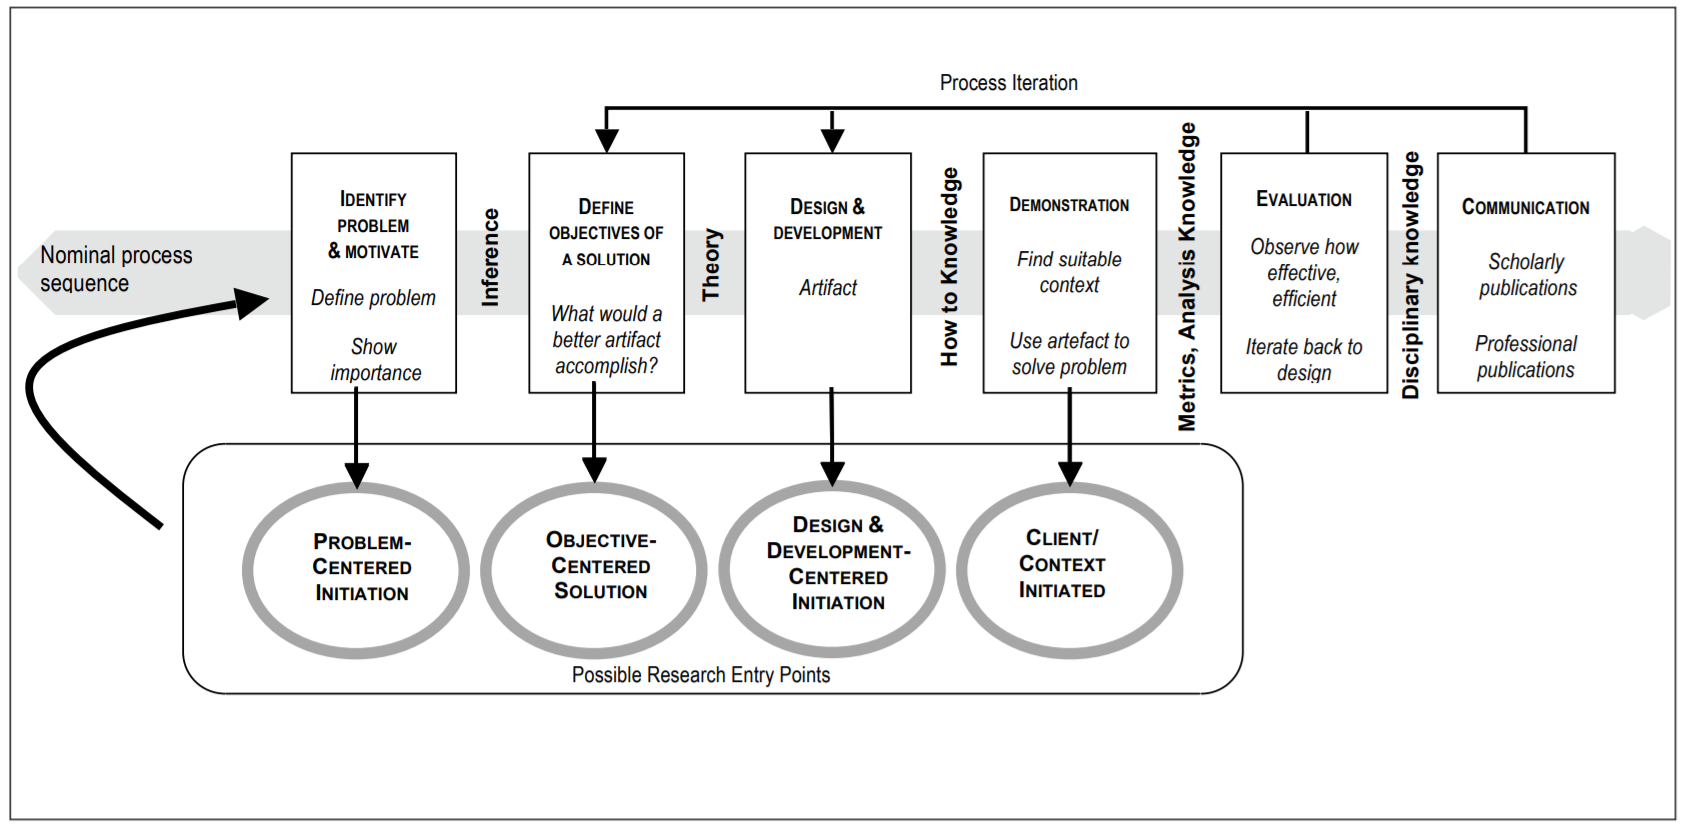
\includegraphics[width=\linewidth]{figures/DSRMPeffers.PNG}
    \caption{Design Science Research Methodology, ~\cite{Peffers2007}}
    \label{fig:DSRMPeffers}
\end{figure}

\subsection{Problem identification and motivation:} 
The process of identifying vessels with an abnormal behaviour, is a complex task. This is mainly because in vessels, abnormal behaviour can be caused by numerous different causes.
  
The authors ~\cite{Laxhammar2008} define Anomaly Detection (AD) as "a method for separating an often in-homogeneous and hard characterized minority of data from a more regular majority of data, by studying and characterizing the majority, so that data in the minority appears as deviations from the patterns found in the majority". 

The main focus of this work is the research and develop of methods that represent vessel motion data, in ways that anomalies can be found.

The MARISA project involves 22 organizations completely motivated to fulfill the overarching objective. 

With the current needs of a more comprehensive approach at the European seas, new and more efficient methods that promote the information exchange between European Union countries, optimizing the European maritime area surveillance and its maritime borders are a current need.

The MARISA project is funded under a H2020, which is a financial instrument that promotes innovation through the European Union.

\subsection{Define the objectives for a solution:}
The research problem is defined accordingly with the MARISA project, which can be defined as: 

~\textit{How to create a system that fuses Data from different sources, capitalizing on the large amount of unexploited maritime data, while autonomously identifying Anomalous Vessel Behaviour.}  

Due to the complexity of this main question, it's important to divide it into smaller questions:

\begin{itemize}
\item Which sources are the most viable to gather spatial data from Vessels,
turning it into a sound Data-Set?
\item Which techniques can transform Spatial Data into Sequential Data, thus creating Vessel trajectories?
\item Can previous Algorithms mine trajectory data from AIS sources, finding anomalies?
\end{itemize}

\subsection{Design and development:} In order to achieve the proposed goals and simultaneous contribute to the MARISA project, the two following objectives were created in Design Science Research. These objectives are described as artifacts:

\begin{itemize}
\item \textbf{Data-Set} A solid Data-Set must be gathered and cleaned. Through the MARISA project, the process of obtaining a Data-Set can be prolonged.Thus ways of obtain AIS Data-Sets free of cost must be researched.

\item \textbf{Route Definition} Numerous methods of vessel route definition, are presented in ~\ref{chapter:literatureReview}.
Although, at this moment a method was chosen that represents the route as a whole. Therefore no information is lost. A detailed description of the latter is presented in ~\ref{section: Trajectory Analysis}.
\end{itemize}

\subsection{Demonstration}https://v2.overleaf.com/project/5b094c27dd648c7b207643b4
While the first artifact is a necessity for future work, is on this data-set that future work will be developed. At this moment I'm using a data-set, from the North America region that has 3.3 million AIS messages from various vessels.
All the MARISA requirements, will in an initial phase be developed on this data-set.
\subsection{Evaluation}
The evaluation of the future artifacts, will be firstly conducted by INOV and after by MARISA partners.
Performance assessment of the artifacts, will be considered after the first implementation is concluded.

\subsection{Communication} 
The research is being conducted for the fulfillment of my masters, therefore a dissertation will be presented for the final evaluation. There is the possibility of submitting future articles for publishing, this possibility depends on the MARISA project.

\chapter{Literature Review}
\label{chapter:literatureReview}
\lhead{Chapter 2. \emph{Literature Review}}

Objectives for the MARISA project are well defined. In order to achieve the proposed goals and in preparation for this thesis a vast number of subjects were investigated. An investigation in the following theoretical topics : behaviour analysis, anomaly detection and maritime safety technologies, were the major keywords for this literature review. 

In section \ref{section: Similar Frameworks} an analysis of the principal similar Frameworks found in the Literature, will be presented.
 A brief introduction to the maritime domain, regarding the Maritime Safety affairs is presented in section \ref{section: Maritime Safety}. In subsection ~\ref{subsection: chp2_AIS}, a description of the AIS technology and its use in the Maritime domain is presented.

\section{Maritime Safety}
\label{section: Maritime Safety}

Shipping is most likely, the most international task of all Worlds Industries, because of this international nature. It has long been recognized that improving maritime safety, is more effective if it is  carried out on a international level, than by individual countries acting unilaterally without any co-ordination, ~\cite{IMO2016}.

The UN (United Nations) in 1948, established the International Maritime Organization (IMO), as the first and principal international organization devoted to maritime matters. 

Since it's creation, the IMO has promoted the adoption of 50 conventions and protocols. The IMO has adopted more than 1000 codes and recommendations regarding the maritime safety and security.

The IMO objectives are easily summarized into their slogan : safe, secure, and efficient shipping on clean oceans.

\subsection{Automatic identification system (AIS)}
\label{subsection: chp2_AIS}
While the maritime safety domain is a vast and complex field for this investigation, it is important to focus on the technologies that the maritime domain has presented.

Automatic Identification System (AIS) is used to identify and locate Vessels by electronically exchanging data over high frequency VHF radio bandwidth to, other nearby ships and Vessel Traffic Services (VTS) stations.

The main motivation for the adoption of the AIS was its autonomous ability to identify other Vessels assisting humans with the collision avoidance. It has the ability to detect other equipped Vessel in situations where the radar detection is limited such as around bends, behind hills, and in conditions of restricted visibility by fog, rain, etc, ~\cite{Harati-Mokhtari2007}. 

In 2000, the IMO adopted a new requirement for all ships, to carry an automatic identification system (AIS) that automatically provides the Vessel information to coastal authorities and other Vessels.

This regulation was initially imposed for all international ships with 300 gross tonnage or more and for ships with 500 gross tonnage and upwards navigating not international voyages. After 31 of March 2014 all EU fishing Vessels above 15m, are obliged by the European Commission to install an AIS, ~\cite{EC2018}

The ships information sent over the AIS is classified into three main categories, they are presented in table:
\begin{table}[H]
\centering
\caption{AIS Information Description}
\label{Table: AIS Categories}
\begin{tabular}{|l|l|}
\hline
\textbf{Category} & \textbf{Description} \\ \hline
 & MMSI - Maritime Mobile Service Identity \\ \cline{2-2} 
 & IMO number \\ \cline{2-2} 
\textbf{Static Information} & Call sign and name \\ \cline{2-2} 
 & Type of ship \\ \cline{2-2} 
 & Length and beam \\ \cline{2-2} 
 & GPS Antenna location \\ \hline
 & Draught of ship \\ \cline{2-2} 
\textbf{Sailing Related Information} & Cargo information \\ \cline{2-2} 
 & Destination \\ \cline{2-2} 
 & ETA - Estimated Time of Arrival \\ \hline
 & Position of the ship \\ \cline{2-2} 
 & UTC - Coordinated Universal Time \\ \cline{2-2} 
 & COG - Course Over Ground \\ \cline{2-2} 
\textbf{Dynamic Information} & SOG - Speed Over Ground \\ \cline{2-2} 
 & Heading \\ \cline{2-2}
 & Navigational Status \\ \cline{2-2}
 & Rate of turn \\ \hline
\end{tabular}
\end{table}

Each Vessel transmits specific information related to the Vessel itself, the MMSI represents a 9 digit unique ID number, that every Vessel is assign with.
Most of the information sent over AIS, is automatically generated by the ships sensors such as the GPS and the compass. Thus minimizing the possibility of manipulate this data, although there is still information that is manually inserted by the crew such as the Navigational Status and the Heading.

Ships fitted with AIS are obliged to maintain the AIS in operation at all times. The AIS autonomously broadcast information, every certain time interval, therefore ships ping their AIS information every time interval   There are international agreements, that protect the navigational information.


\section{Behaviour Analysis}
Behaviour Analysis, is a vastly researched topic that involves many research fields. A vast number of Frameworks with the main objective of Maritime Behaviour Analysis are proposed in the literature, some of these frameworks are presented in section ~\ref{section: Similar Frameworks}.

For this work Vessel behaviour is as considered as a baseline in which abnormal behaviour can be found. This baseline occurs as normal trajectories are various and constant, producing a normalcy model of Vessels dynamics in which Machine Learning Techniques can learn.

Anomalies don't necessarily mean that there is something abnormal with the ship Vessel behaviour. That is something hard to imply with only AIS data. Anomalies in the AIS data can represent numerous abnormal events. Some of them that can be illegal, that's why further investigation from maritime authorities is needed. 

\subsection{Similar Frameworks}
\label{section: Similar Frameworks}

There are a vast number of frameworks in which Vessel behavior will be analyze. This will be done with the purpose of anomaly detection which are fully defined as integrated systems. The authors in ~\cite{Lei2016} suggested the framework MT-MAD (Maritime Trajectory Modelling and Anomaly Detection), in which a given set of moving objects, the most frequent movement behaviour are explored, evaluating a level of suspicion hence detecting anomalous behaviour.

The authors in ~\cite{Pallotta2013}, introduced the framework TREAD (Traffic Route Extraction and Anomaly Detection). The framework is proposed in which an Unsupervised Route Extraction is used to create a statistical model of maritime traffic from AIS messages, in order to detect low-likelihood behaviours and predict Vessels future positions.

A framework for Vessel behaviour analysis focusing on Vessel interaction or rendezvous. The proposed framework, is divided into the following three logical connected phases: Engagement Detection, Scenario  Detection and Anomaly Detection. The use of the 3-phase framework serves as a filter to reduce the volume of data that is processed by the sub-sequential phase. Therefore prioritizing critical scenarios, that request human intervention ~\cite{Shahir2015}.

Although accessing the performance of the frameworks, is an ardours task. There is no defined benchmark set where tests can be performed, with labeled samples described as positives or negatives of what are considered anomalies at seas ~\cite{Laxhammar2008}. 

In~\cite{Mao2016}, a detailed solution for constructing an AIS database, with the potential value for being used as benchmark database for maritime trajectory learning, and efficiency testing of data mining algorithms.

A partition-and-detect trajectory in which trajectories are partitioned into a two-level of granularity achieving high efficiency and high quality trajectory partitions, therefore detecting outlier trajectories using density-based methods, ~\cite{Lee}.

There are numerous studies that show how, Vessels tend to alter their routes in order to achieve safe distances when passing near other Vessel. In ~\cite{2017Offshore} a detailed study on Merchant Vessels AIS data, presents how this type Vessels alter their route, when new surface offshore petroleum installations are constructed.

\section{Trajectories Analysis}
\label{section: Trajectory Analysis}
Trajectories analysis is a researched field for numerous years. It is researched in areas where moving objects, this objects can be Humans, vehicles, animals, or even natural events such as hurricanes or storms.
A survey of trajectory data analysis applications, is presented in ~\cite{Feng2016}.

As the volume of positional AIS data exponentially increasing, it is important to find methods in witch raw trajectories data can produce value. This methods that learn with trajectory data can greatly impact the Maritime domain.

Trajectory learning is the process of learning motion-patterns from trajectory data using unsupervised techniques, mainly clustering algorithms ~\cite{LeGuillarme2013}.
Morris and Trivedi ~\cite{Morris2008}, further categorize trajectory learning as a three-step procedure: 

\begin{enumerate}
\item Trajectory Pre-Processing.
\item Trajectory Clustering. 
\item Path Modelling.
\end{enumerate}

In the Maritime domain, as Vessels are free to navigate in open waters, this fact produces a specific level of uncertainty related to Vessel trajectories, there are no standards for Vessel trajectory representation.

A way to discretize a trajectory discovering frequent regions is presented in ~\cite{Lei2016}. Representing the trajectories in a spatial grid in which a cell represents a geographical area with a defined size.

Pallotta, proposed a method that enriches the raw Vessels tracks with a description of the ship movements. This is the raw trajectories are labelled with the Vessel movement type information as 'Stationary' or 'Sailing' ~\cite{Pallotta2013}.

The authors in ~\cite{Lee}, raw trajectories are partitioned into sub-trajectories, creating a new insight for data analysis, adding the possibility of focused region analysis.  

A framework for scene modelling using trajectory dynamics analysis, for the discovery of POIs(Point of Interest) and the learning of AP(Activity Path), ~\cite{Morris2008}. 
These last representation is quite important for the Maritime domain, as the discovery of new POIs, can indicate the common Vessel destinations (e.g. frequent fishing zones, ports, etc.).  

\section{Time Series}
\label{section: Time Series}
The concept of time series is related to trajectories, as a time series is a set of ordered observations on a a quantitative characteristic of a
phenomenon at spaced time period, ~\cite{Ivanovic2016b}. Formally, a uni-variate time series $xj$, is defined as a sequence of real numbers, where $n$ is the length of the series, represented as:

\[xj = \left \{ x(i) \in \mathbb{R}: i = 1,2,3,...,n \right \} \]

 There are numerous applications for time series analysis, one of the main applications, is the use past time series, in order to forecast future values. These applications are used in numerous areas such as economics, engineering and others.


\subsection{Multivariate Time Series}
The AIS data cannot be described as a uni-variate times series, as it is composed by various variables. Therefore AIS data needs to be analyzed as a Multivariate Time Series (MTS).
For each AIS message, the features can be extracted with the timestamps that the message was broadcast. A detailed description of the AIS features is found in section ~\ref{subsection: chp2_AIS}. 

A possible representation of a Multivariate Time Series, $X$ is:
\[ X = (x_{1}, x_{2}, x_{3}, \cdots,x_{m}) \]

Where each $xj$ is defined in section ~\ref{section: Time Series}.

\[ Xj = \left \{ Xj(i) \in \mathbb{R}: i = 1,2,3,...,n \right \} (j = 1,2,3) \]

The analysis and classification of MTS is a arduous task for traditional machine learning algorithms, mainly because these algorithms do not handle well dozens of variables, ~\cite{MTS1}. Representing MTS into multiple univariate time series, can create losses in the correlation of these variables, as variables are being processed them independently.

\subsection{Time Series Clustering}
Temporal data mining research, a big emphasis lies on the clustering, and posterior classification of time series data. Time Series Clustering is used to identify in data-sets, homogeneous groups where same group object similarity is maximized, and the minimized when not in same group.  

The authors in ~\cite{WarrenLiao2005}, summarize previous work that investigates the clustering of time series applications in various fields, and propose an extensive survey. 

The same authors, define a necessity to clustering, when working with unlabelled data. This data can come from various sources including : categorical, numerical, images, spatial, e.t.c.

The main source of data for this work is AIS data, which is a  unlabelled multivariate data source. Labelled AIS data-sets for anomaly detection are either really expensive, or just not available for the public domain.  


\begin{figure}[H]
	\centering
	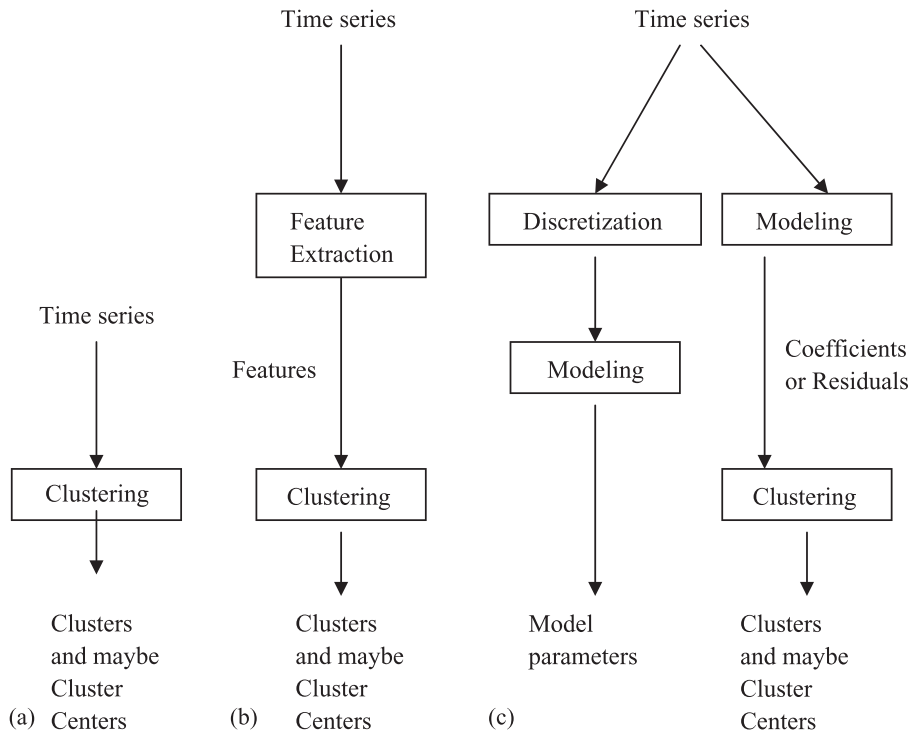
\includegraphics[scale = .6]{figures/TimeSeriesClustering}
    \caption{Three types of time series clustering defined in, ~\cite{WarrenLiao2005}}
    \label{fig:TimeSeriesClustering}
\end{figure}

Time Series Clustering can be categorized into three main general approaches, simply described in figure ~\ref{fig:TimeSeriesClustering}, these categories being:

\begin{itemize}
\item \textbf{Raw-data-based approaches (a)} These approaches work with raw sets of data, normally in the time domain. 

\item \textbf{Route Definition} Several methods of Vessel route definition, are presented in~\ref{chapter:literatureReview}.
Although, at this moment a method was chosen that represents the route as a whole. Therefore no information is lost, a detailed description of the latter is presented in~\ref{section: Trajectory Analysis}.

\item \textbf{Model-based approaches} This is a more complex clustering technique, in which, each Time-Series is considered as a statistical model or as a mixture of statistical distributions, thus two time series are considered similar when the models that fit this distributions are similar. 
\end{itemize}


%\todo{Needs completion for future work.}


\subsection{Time Series Classification}
Time series classification, is used for numerous purposes, from, the main difference when classifying or clustering Time Series lays in the fact that, classification can occur when a predefined set of classes already exist and the main objective is to classify this data in the different classes, thus in machine learning being considered a Supervised Learning task. 

Early work, from 1998, the authors propose p-value hypothesis test, performed for every pair of stationary multivariate time series, ~\cite{MTS1999}.

Three main categories of sequence time series classification, are defined by the authors in ~\cite{MTS_Classification}:

\begin{description}
\item[Feature Based Classification] A sequence of features is transformed into a feature vector, then convectional classification methods are applied. Feature selection represents is an important task for this method of classification.

\item [Distance Based Classification] The distance function that measures the
similarity between the time series, induce the quality of the classification overall. A more detailed research on these distances is presented in \cite{Knorr2000}.

\item [Model Based Classification] Where models, such as multivariate Gaussian mixture model (GMM) ~\cite{Laxhammar2008}, Support Vector Machines (SVM) or Hidden Markov Models (HMM) and other statistical models are used to classify time series.

\end{description}
 

\section{Distances Measures}
In order to compare classify a time series using distances, the concept of distance, and type of distance must be defined.

A distance is defined as a numerical measurement, that measures how far two objects are from each other. There are a vast number of distances used in computer algorithms. The most commonly used distance measure is the Euclidean distance, this measurement is a metric distance function, since it obeys to the three fundamentals metric properties: non-negativity, symmetry and triangle inequality ~\cite{Cai2004}. 

The similarity between two time series, can be calculated by simply summing the ordered point-to-point squared distance between both time series, this is shown in figure ~\ref{fig:EuclidianDTW}. 

Although, euclidean distance between two time series can only be calculated if, both time series are of equal length, ~\cite{EuclidianRef}. 
If two time series are identical, but one is shifted slightly along the time axis, using the Euclidean distance, it may consider the time series very different from each other, ~\cite{Salvador2007}.

This creates a problem when analyzing certain type of time series, as both may not have them same length, or might just be time-shifted, which happens when analyzing AIS data. In the literature a few solutions are presented, one of them is using another distance measure. 

\begin{figure}[H]
	\centering
	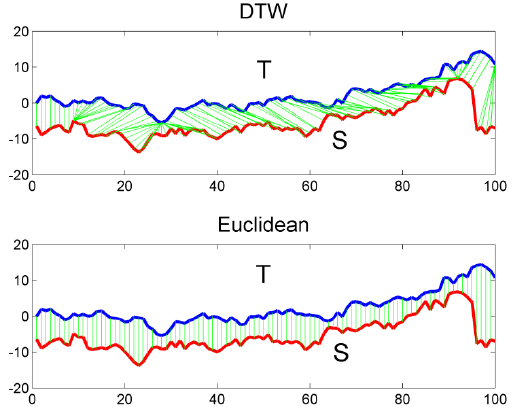
\includegraphics[scale = .5]{figures/DTWEuclidean.png}
    \caption{Difference between DTW distance and Euclidean distance (green lines represent mapping between points of time series T and S),~\cite{EuclidianRef}}
    \label{fig:EuclidianDTW}
\end{figure}


\subsection{Dynamic Time Warping (DTW)}
Dynamic Time Warping (DTW) is a algorithm that computes the optimal alignment and distance between two time series, ~\cite{Seto2015}. One time series may be “warped” non-linearly by stretching or shrinking it along its time axis.
%[GET A BETTER REF FOR THIS, NOT SALVADOR].

Although computing the DTW between two time series, is quite computationally expensive, has it's time and space complexity is $O(N^2)$, that limits its usefulness to only small time series with no more than 1000 points, ~\cite{Salvador2007}. 

As distance measures play an important role for similarity problem, in data mining tasks.








%\section{Data Fusion}
%\todo[inline]{Needs completion for future work. Depending on future work this might be needed.} 




\chapter{Modular Anomaly Detection Framework}
\label{chapter:Chapter 3}
\lhead{Chapter 3. \emph{Methods and Systems Developed}}

In this Chapter, we present the overall description of steps towards the development of the \emph{Modular Anomaly Detection Framework} which is be used throughout this dissertation. 
A crucial component in this work relied on a technically accurate definition of a \emph{maritime anomaly}. This is generally speaking a challenging task since a data-driven definition is currently lacking or insufficient. A more meaningful solution to this problem was provided by the aid of maritime experts who were engaged in the \textsc{Marisa} project. In particular, members of the Portuguese Navy interacted with us in order to offer the required their exclusive technical insight.

Given their specific input and real-world knowledge of the maritime domain, one can arrive at a well-defined concept of anomaly that can be translated into a precise notion to be used in this Framework. Before we engage in the specific requirements that served as a blueprint for the developed framework, such a definition will be given. This will then be followed by the technical description of such requirements, namely by distinguishing \emph{anomaly} and \emph{data requirements}.

Lastly, a general overview of the proposed Modular Anomaly Detection Framework, which will be referred to as MAD-F from now on, is presented. This is done in light of Figure~\ref{fig:Framework}, whose modules are explained individually throughout the following Subsections~\ref{subsection: Data Ingestion},~\ref{subsection: 3 Pre-processing},~\ref{subsection: 3 Feature Engineering}, ~\ref{subsection: 3 Vessel Trajectory Extraction},~\ref{subsection: 3 ADS} and~\ref{subsection: 3 RB-ADS}.


\section{Anomalies within the MAD-F}
\label{section: Framework Requirements}
An anomaly may have numerous interpretations depending on the context in which it is found. However, it can be generally conceptualised as a subset of data that stands out in some preconceived way when contrasted to the overall dataset. Nowadays, the anomaly detection of vessel behaviour is solely done by human maritime experts. This procedure depends on national security agencies. Within their duties, these agencies are responsible for assuring the coastal surveillance of their territory by assessing possible threats and identifying abnormal behaviour. The current methods employed by these institutions are neither efficient nor scalable and therefore not suitable for the challenges brought by the exponential growth of vessels at seas. This state of affairs creates an ideal situation for the use of data-driven models to assist the maritime experts.

The notion of anomaly just presented is unsatisfactory given both the complexity and purpose of the problem. For the goals of this project, such a technical definition is tailored specifically by the maritime agencies involved in the \textsc{Marisa} project and we therefore refrain from applying our own definitions, which usually stem from abstract statistical data-driven notions. 

By having meetings with maritime experts a list of the anomaly requirements was agreed. For this work this list served as not only the concrete anomaly requirements, but also as a guide for the overall implementation of the \emph{MAD-F}. The list of anomaly requirements in shown under in Table~\ref{Table: Anomaly Requiremtens}.

\begin{table}[H]
\centering
\caption{MAD-F anomaly requirements, which were defined by maritime officers.}
\label{Table: Anomaly Requiremtens}
\begin{tabular}{@{}ll@{}}
\toprule
Anomaly Requirement & Provided Description \\ \toprule
\textit{\textbf{AR1}} & \begin{tabular}[c]{@{}l@{}}Detect Abnormal changes of \\ (more than a configurable value) Direction.\end{tabular} \\ \midrule
\textit{\textbf{AR2}} & \begin{tabular}[c]{@{}l@{}}Detect Abnormal changes of \\ (more than a configurable value) Velocity.\end{tabular} \\ \midrule
\textit{\textbf{AR3}} & \begin{tabular}[c]{@{}l@{}}Detect Vessels disappearance from sensor \\ coverage for more than a configurable Time Period.\end{tabular} \\ \midrule
\textit{\textbf{AR4}} & \begin{tabular}[c]{@{}l@{}}Detect when the observed \\ Vessel Navigational Status is not consistent \\ with the reported Vessel Kinematic features.\end{tabular} \\ \midrule
\textit{\textbf{AR5}} & \begin{tabular}[c]{@{}l@{}}Detect when Vessels report a \\ geographical and time incompatibility.\end{tabular} \\ \midrule
\textit{\textbf{AR6}} & \begin{tabular}[c]{@{}l@{}}Detect when two or more Vessels are \\ approaching close to each other.\end{tabular} \\ \bottomrule
\end{tabular}
\end{table}

As mention previously, requirements for this work were distinguished from anomaly requirements and data requirements. The latter was intrinsic for this work, as the uncertainty of data types and sources when dealing with the maritime field is immense. The problem of having numerous types and sources of data is still aggravated as the maritime domain is also capable to produce enormous workflows of data. Thus, a specific data requirement for this work could be simply specified as: 

\emph{The developed Framework, must be able to ingest fuse and store different sources of maritime Data, while also handling enormous workflows of data in real-time.}

\section{Modular Vessel Anomaly Detection Framework}
In order to develop a Framework capable of achieving the requirements defined above in Section~\ref{section: Framework Requirements}, we propose the Modular Vessel Anomaly Detection Framework. The \emph{MAD-F} is able to ingest data from different feeds in real-time data while simultaneously constructing a Data-Base for Vessels Trajectories in a unsupervised manner. Anomalies are then detected in a offline manner from the saved trajectory data, or online in real time addressing the incoming streams of Vessel Data. 
The framework was developed to be modular as there are either no inputs or outputs standards for the Maritime Domains. Thus, by providing a configurable and not static framework, we give the configuration flexibility for the \emph{MAD-F} being configured for different scenarios or even different National Maritime Authorities, or even to new Modules being added in the future.
In Figure~\ref{fig:Framework} we present the architecture of the \emph{MAD-F} and the following subsections will discuss each of the framework modules: Data Ingestion, Data Pre-processing, Feature Engineering, Trajectory Extraction and both anomaly detection modules : Anomaly Detection Service and Rule Based Anomaly Detection Service.
\begin{figure}[H]
\centering
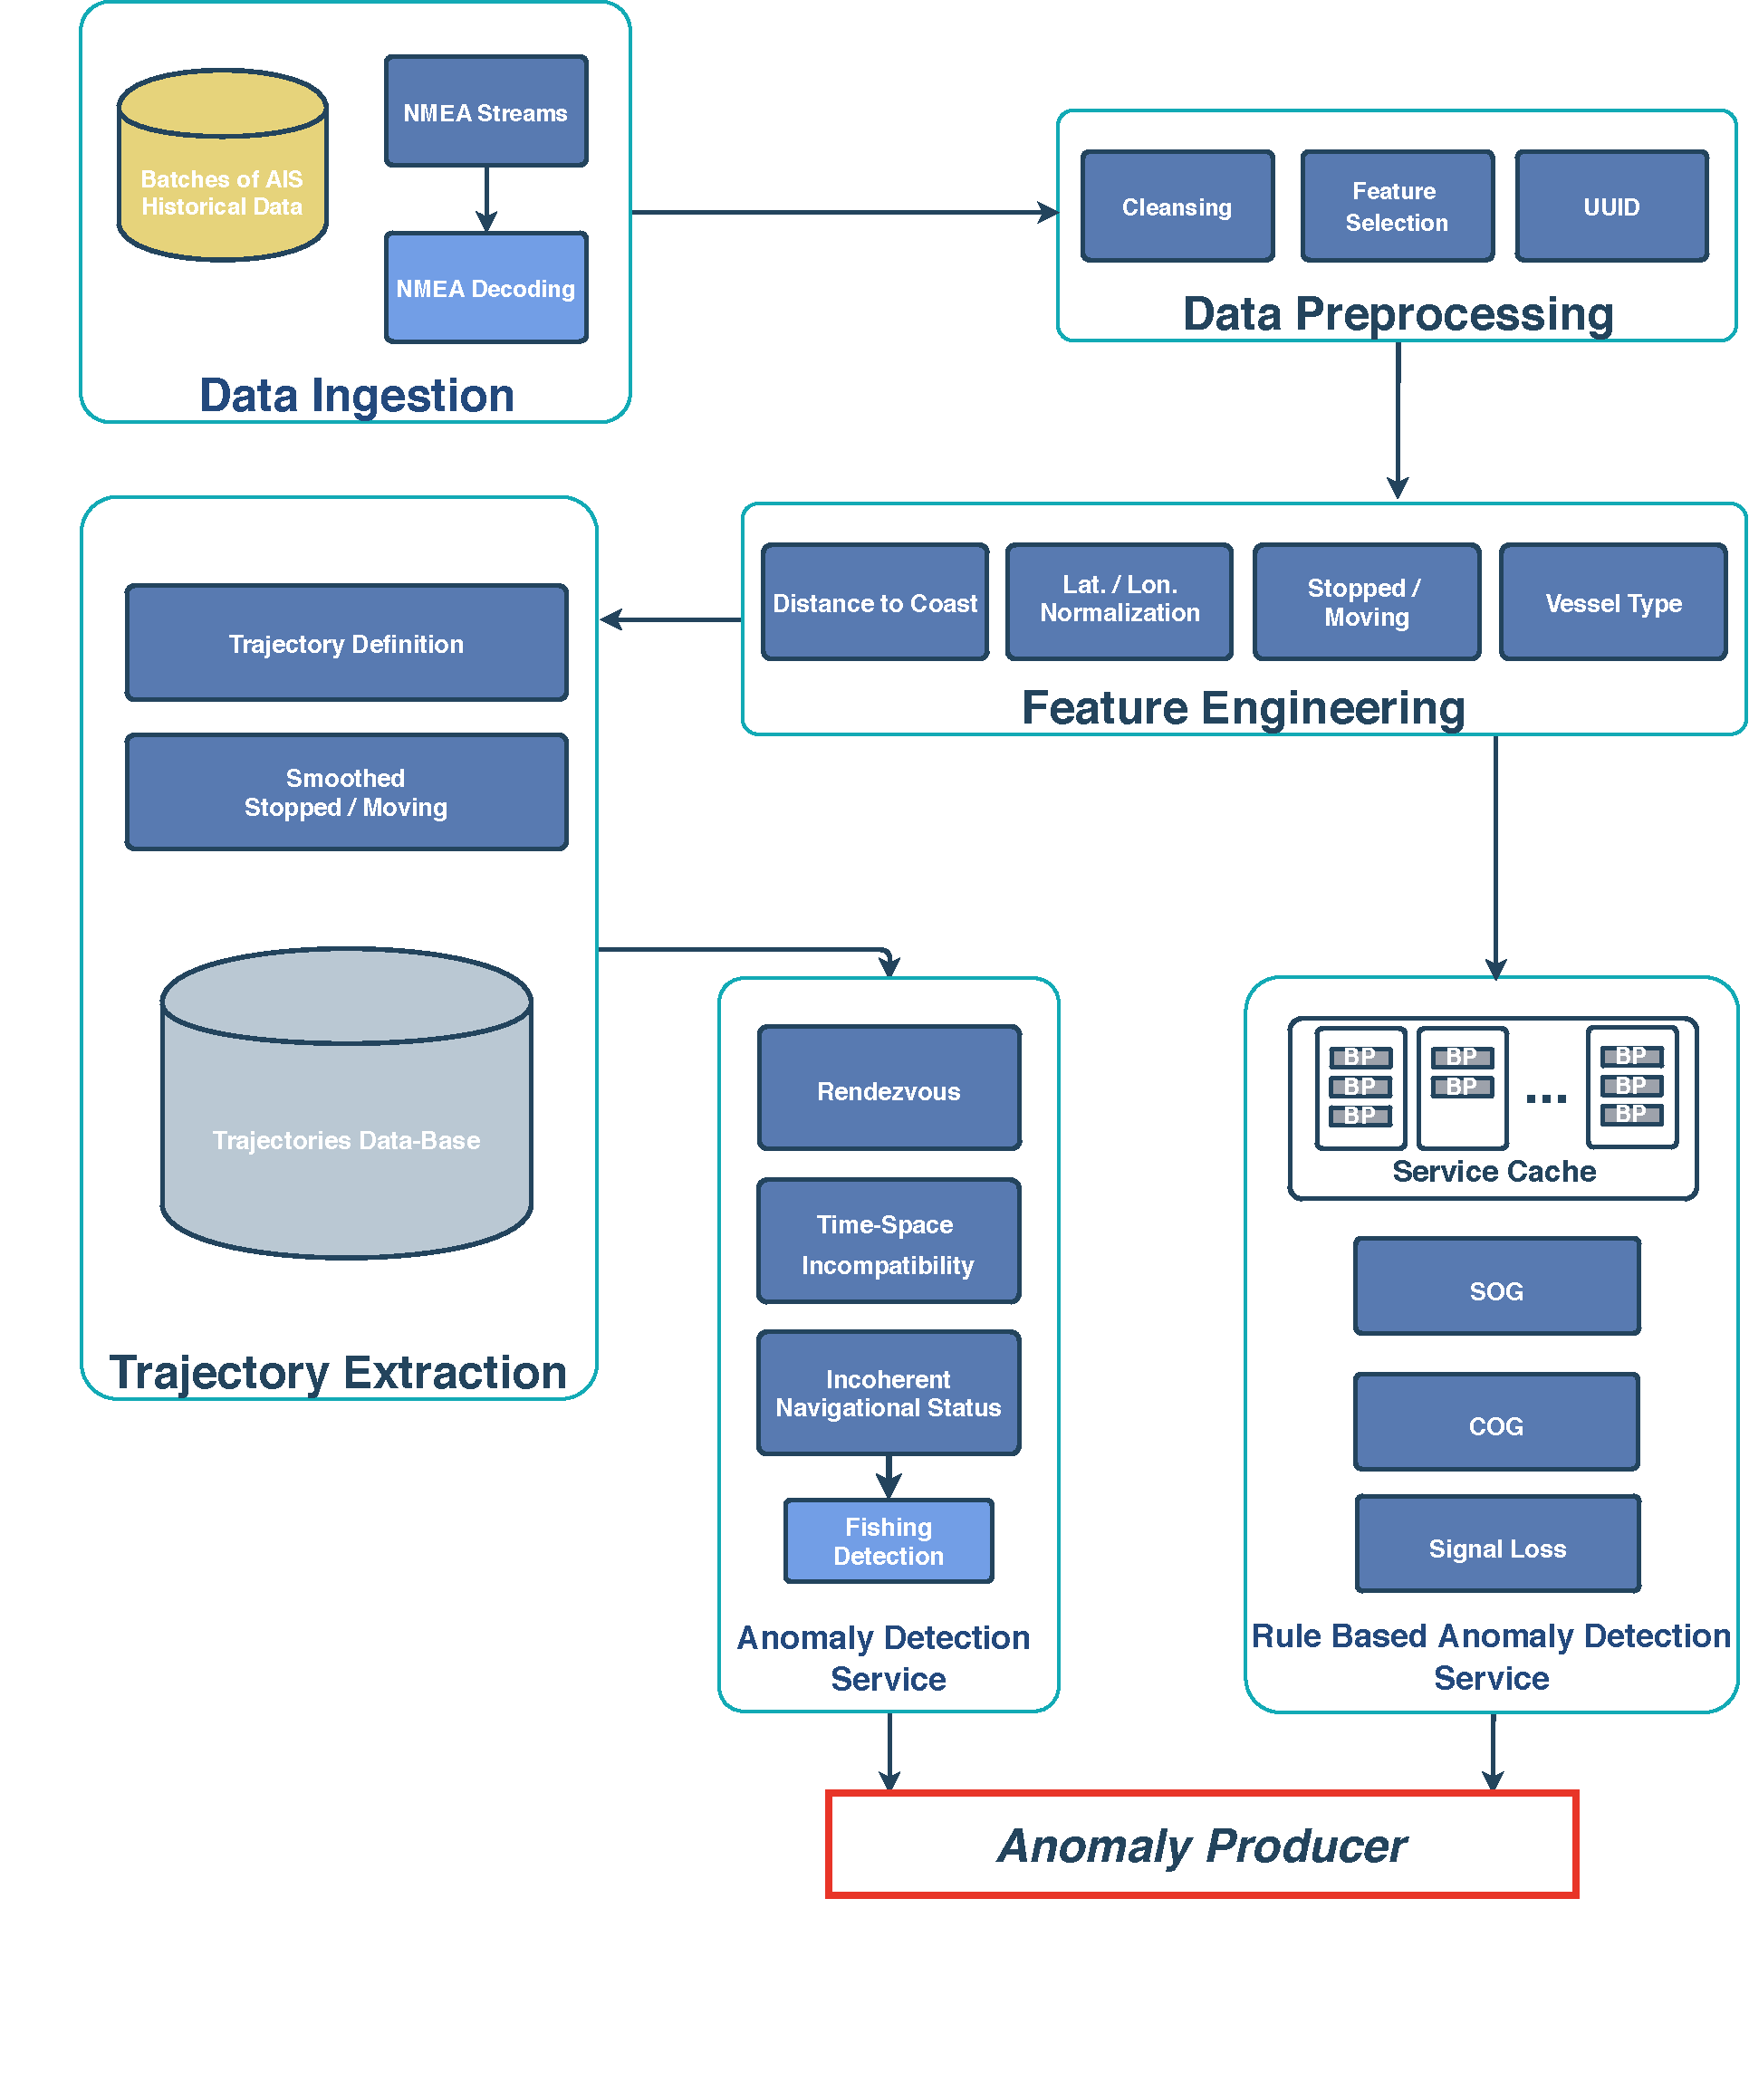
\includegraphics[width=\textwidth]{figures/Ch3/Framework.pdf}
\caption{Proposed architecture for the \emph{MAD-F} Framework}
\label{fig:Framework}
\end{figure}

\subsection{Data Ingestion}
\label{subsection: Data Ingestion}
Data Ingestion Module, represents the Data input for the developed Framework. AIS data was the most representative data type used for this work, as it showcases the actual instantaneous Vessel information.
Although, used AIS data for this work came in two really distinct formats. It came either in \emph{Historical Batches} representing Historical sets of Data, or real \emph{NMEA AIS Streams} which represent real, real-time data. For both data formats, the framework is scalable, and able to ingest one or multiple feeds / sources of data simultaneously.

%AIS Historical Data-Sets, can be found in open-access repositories, although Historical AIS Data providers cap the frequency of the messages transitions. This drastically reduces the number of transmitted messages, but also reduces the overall detail of the Data, as lower transmissions rates produce a less certainty of the movement presented by each Vessel. Which, for most general uses of AIS (e.g. managing a fleet, estimations of time of arrival ...), transmissions rates of 3 Seconds vs 30 Seconds, do not provide any information gain, as Vessel kinematics tend to not change abruptly in short periods of time. 

Via the \textsc{Marisa} project, we accessed AIS live feeds from antennas all around the Portuguese coast line. This Antennas receive Vessels transmissions via AIS up to 20 Nautical Miles of the shore depending on the weather conditions, and with reception rates up to 30 Messages per minute per vessel. The real live feeds of AIS data, are received via TCP in the NMEA format.

National Marine Electronics Association (NMEA) is a standard communication protocol used by Maritime Sensors such as Accelerometer, Giroscope, GPS receivers, etc.
NMEA encapsulates the information from the different Vessel sensors, and broadcasts this information to coastline antennas and nearby Vessels via AIS protocol.

\begin{figure}[H]
\centering
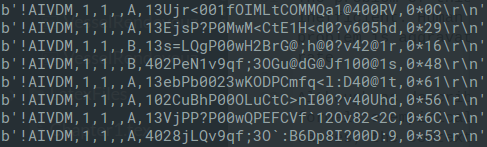
\includegraphics[scale = .55]{figures/Ch3/NMEAexample.png}
\caption{Snapshot of raw AIS data in NMEA format.}
\label{fig:NMEAexample}
\end{figure}
%Via the project, we had access to multiple live NMEA feeds, as a way to not only validate our developed methods with live feeds of Nautical data, but also to produce methods that were capable of handling the scale of data that is produced by National feeds.
Although the use of real AIS data comes with many challenges, as it is mandatory to decode, sort and store the received data, thus allowing the incoming data to be used as viable source of data. Secondly, as AIS-receiving stations receive the broadcast AIS information from multiple AIS-equipped vessels simultaneously, and the reception range of each AIS-receiving can vary depending on the actual weather conditions and the location of where such station is located. This originates two main problems :
\begin{enumerate}
\item Duplication of reception:  With the variation of reception ranges from the AIS-receiving stations, this creates the problem of multiple stations receiving the same vessel broadcast. The duplication of messages is a problem which occurs when handling real NMEA streams, the methods used to solve such problem are presented in Section~\ref{subsection: ch4 Data Ingestion}.

\item Non-reception of broadcast: Similar to the problem presented above the non-reception of by any receiving station can also occur. To address this problem, Maritime Agencies use satellite AIS (S-AIS). S-AIS solves the problems related to the reception range, but presents another problem with refreshment rates, has the reception of the broadcast are dependent of satellite revisit time \cite{Robards2016ConservationReview}. 
\end{enumerate}


%when dealing with real-time NMEA feeds as
%the reception range of the AIS receiving antennas varies depending on weather condition when this antennas receive information from multiple Vessels two more common problems can occur:


%. Normally, AIS-Receiving stations are antennas located along the coast line in high grounds, the reception range of these antennas vary, mainly depending on distance to shore, the elevation in which the antenna is located, and the antenna type itself.

%Although, the distance in which Stations are capable of receiving AIS messages presents a problem to the Data, as reception ranges vary from 15 Nautical Miles to 50 Nautical Miles, which creates the problem of 



%\subsection{Data Storage}
%With NMEA streams producing enormous workflows of data, the storage of becomes a problem for the developed Framework, as it must not only decode and process the NMEA feeds but also store the decoded messages, in a "very fast" and scalable way.

%Thus, and as requirement of the MARISA project was to use Apache Spark [REF FOR APACHE SPARK] modules for data-ingestion and pre-processing, we decided to use Apache Cassandra as the Data-Storage for the proposed framework.

\subsection{Data Pre-processing}
\label{subsection: 3 Pre-processing}
The Data Pre-processing module, is the first step of Data Wrangling in our Framework, the motive for this module is to select, transform, and clean the received data, incoming from the Data Ingestion Module. 
As described in Section~\ref{subsection: chp2_AIS}, AIS presents a large amount of different features, which can be used for different problems. Feature Selection represents a important step for this work. This work being partially a unsupervised learning problem, the selection of the "relevant" features directly influences the overall performance of the \emph{MAD-F}, but also the expected results from the learning task. Such representative task requires pre-conceived knowledge of Vessels dynamics and behaviour, which is only gained with experience in the Maritime Domain. For this work the feature selection was done based on the literature, and also by accessing Maritime Expert Knowledge via the \textsc{Marisa} project.

During the \emph{Pre-processing}, a data-cleaning process is conducted, discarding corrupted data. This is done based on the information that standardises the AIS features, which is further detailed in Section~\ref{section: Data Analysis}.

Most importantly, in this module the concept of \emph{Behavioural Point} is defined. \emph{Behavioural Point} which will be referred as $BP$ from now on, for this work represents our normalised representation of the previously selected features. A detailed explanation of this concept is provided in Subsection~\ref{subsection: Behavioural Point}.

\subsection{Feature Engineering}
\label{subsection: 3 Feature Engineering}
Feature Engineering, represents the second step of Data Wrangling for the proposed Framework. During this step, the already pre-defined $BPs$, in the Data Pre-processing module, are enriched by extrapolating additional features. 

Firstly for each $BP$ received by this module, if the Vessel Type is not received in the AIS message, the Vessel Type is either extracted from external Vessel Information Sources, or it is scrapped from this internet.
Secondly, each $BP$ is enriched with by calculating the closest country and respective distance to Shore. The same is done to Ports, by calculating the distance to the closest Port. Also, in this module with the reported kinematic features, the instantaneous move state of the vessels is inferred.

This procedures are further individually explained throughout Subsections~\ref{subsection: Vessel Type},~\ref{subsection: Distance to Coast},~\ref{subsection: Stopped/Moving}.

%presents a crucial step for any machine learning project, as 

%selecting the right features to represent the data, directly influences any result generated by the Anomaly Detection Modules.  

%We further enrich our features in two ways, firstly by analysing each AIS message as a single point in Time and calculating additional distances, such as distance to Shore and distance to the most near Port.

%each point in t the represented features of each message by by doing a point based analysis, in which we considered the information of  

%by normalizing the Latitude and Longitude features of each position, calculating the Distance to Shore and the kinematic features that represent the instantaneous move-state of the Vessel. Every calculation is done a priory, thus enhancing the performance and reliability of the Anomaly Detection Modules, which are explained in detail in section \todo{REF TO SECTION!}

\subsection{Vessel Trajectory Extraction}
\label{subsection: 3 Vessel Trajectory Extraction}

Vessel Trajectory Extraction module, handles the definition, storage,  updating and inserting of new incoming $BPs$ into defined \emph{Trajectories}.
When considering Trajectories, the $BPs$ stop being valued as single points in Time, and the aggregation of $BPs$ via the Vessel Identifier throughout time, start representing a Vessel Trajectory. This allows a more conclusive Vessel behaviour analysis based on its past trajectory. Although, in order to work with Trajectory, such concept needs to be defined and represented in a optimal manner. Furthermore, when dealing with real Maritime data (and specially when working with real Maritime Authorities) it is extremely important to trace-back/log of the data, from which, justifying generated anomalies is possible. 
In Section~\ref{subsection: Trajectory Definition} our definitions of a vessel trajectory. 

%Behaviour analysis based on the past historical Trajectory data. Analysis of Trajectories drastically increases the level of complexity, when compared to analysis points, thus it is required quick and efficient representation of a Trajectory.

\subsection{Anomaly Detection Service}
\label{subsection: 3 ADS}
ADS (Anomaly Detection Service) Module, represents for our Framework the Batch Layer for Anomaly Detection Services. \emph{ADS} module works offline in effective time, on batches of historical Trajectory Data served from \emph{Trajectory Data-Base} from the \emph{Trajectory Extraction} module. Access to Trajectory Data, is done by querying the \emph{Trajectory Data-Base} with a configurable set of parameters, which can be time restrictive(such as the 10 past Hours) and or from a Vessel specific set of Vessels. 

Received Trajectory Data, is then used to detect: \textbf{Time Space Incompatibility}, \textbf{Vessels Rendezvous}, and \textbf{Incoherent use AIS Navigational Status}. For the latter, we create a sub-method for the detection of \textbf{Fishing Activities} based on Vessels characteristics and Dynamics and the reported Navigational Status.
The implemented methodology for the detection of each Anomaly is represented in Subsections~\ref{subsection: 4 Time-Space Incompatibility},~\ref{subsection: 4 Navigational Status Validation},~\ref{subsection: Fishing Activity Detection} and~\ref{subsection: 4 Vessel Rendezvous} respectively.


\subsection{Rule Based - Anomaly Detection Service}
\label{subsection: 3 RB-ADS}
RB-ADS (Rule Based - Anomaly Detection Service), opposed to the ADS module described above, corresponds to the Speed Layer for the Anomaly Detection Services. \emph{RB-ADS} modules works online in near real-time, accessing the stream of already pre-processed $BPs$ from the Feature Engineering Module. In order to the \emph{RB-ADS} be able to perform Anomaly Detection in near real-time, a Queuing Systems for this module was defined, which we named \emph{Service Cache}, which we further explain in Section~\ref{section: 4 Rule Based Anomaly Detection}. The arriving stream of $BPs$, is are stored in individual Vessel Queues of size $N$. The individual Queues are then accessed, allowing a real-time calculation of the set of Anomaly which can be defined by Rules. The Anomalies validated online trough rules for this work are: Abnormal change of Velocity and Direction (Anomaly Requirements 1 and 2 respectively) and Vessel Signal Loss (Anomaly Requirement 3), our approach towards the detection of such anomalies is described in Section~\ref{subsection: 4 Course}  


%This was if i talked about AIS SIGNAL LOOS HERE
%Ships equipped with AIS are obliged to keep the AIS autonomously transmitting AIS messages. A way that ships illegally hide their position and possible what the ships is doing objectively, is by switching off the AIS, or finding ways to block the communications of the AIS transmitter with the coastal receivers.

%This creates a problem in the maritime domain, has maritime authorities are constantly finding new ways to discover this illegal activities. A method that looks into historical or new streams of ata, was developed. 

%\subsection{Time Series Analysis}

%\subsection{Anomaly Producer}
%Anomaly Producer, serves for this Framework as exit point for the MAD-F.This module communicates with other outside services by producing anomalies generated by the Anomaly Detection modules from the Framework. As for this present work, due to the Marisa duties we did not develop any anomaly visualisation module. This module produces anomalies, in the normalised MAD-F anomaly format which we will discuss in Section XX.

\addtocontents{toc}{\vspace{2em}}

%-------ANEXOS---------

%\appendix
%\appendixpage
%\addappheadtotoc

%\chapter{Appendix's title}
%\label{AppendixA}
%\lhead{Appendix A. \emph{Appendix's title}}


\addtocontents{toc}{\vspace{2em}}
\backmatter

%-------BIBLIOGRAFIA---------
%Adicionem as referências em BibTeX ao ficheiro references.bib
\label{References}
\lhead{\emph{References}} 
 
%\bibliographystyle{plain}
%\bibliographystyle{ieeetr}
%\bibliographystyle{ieeetr}

\bibliographystyle{unsrt}
\bibliography{ThesisReferences}

\end{document}